\documentclass[12pt]{article}
\usepackage{geometry} 
\geometry{a4paper}                   % ... or a4paper or a5paper or ... 
\usepackage{graphicx}
\usepackage{amssymb}
%\usepackage{MnSymbol} % for \rcirclearrowleft
\usepackage{epstopdf}
\usepackage{fancyvrb}
\DeclareGraphicsRule{.tif}{png}{.png}{`convert #1 `dirname #1`/`basename #1 .tif`.png}

\def\name#1{\textbf{#1}}
\def\mycaption#1{\sf\bfseries\caption{\sf #1}}
\makeindex
%set-tag \seen{}

%==========================================================================================================
% Additional Packages (Dave)
\usepackage{siunitx, booktabs, cancel, csquotes, mathpazo} % Allows correct typesetting of SI Units
\usepackage{todonotes} % allow in-text and marginal comments for draft manuscript
\usepackage{url} % allows typesetting of web addresses etc.
\usepackage{cite} % groups multiple citations together seperated by hyphen e.g. \cite{1},\cite{2},\cite{3} => [1-3]

%==========================================================================================================

%\usepackage{euler}\usepackage{beton}\usepackage{sectsty}\allsectionsfont{\mdseries}
\makeatletter
\def\labelNum#1#2{
	\protected@write\@auxout{}{\string\newlabel{#1}{{#2}{?}}}
}
\makeatother

%generate relit-def.tex ., /ends/-1, \unseen{}
\iftrue
	\makeatletter
	\def\@uc#1{\uppercase{#1}}%
	\def\relitindex #1 #2 {\immediate\write\@indexfile{\string\indexentry{\@uc Relit #1!#2@{\string\texttt{#2}}}{\thepage}}}%
    \def\manualrelitindex #1 #2 {\immediate\write\@indexfile{\string\indexentry{\@uc Relit #1!#2@{\string\texttt{#2}}|manualrelitpage}{\thepage}}}%
    \def\manualrelitpage#1{#1*}
      \expandafter\DeclareRobustCommand\csname relit\endcsname{\@ifnextchar[{\@@relit}{\@relit}}
      \def\@@relit[#1]#2{%
      	 \def\seen{{\tt\char'134}seen\{\}}%	
         \def\unseen{{\tt\char'134}unseen\{\}}%	
        {\setbox0=\hbox{\relitindex #2}\par\noindent\tt\hskip -1em\textcolor{red}{*~RELIT: #2, #1}\vskip 0pt}%
        	 \marginpar{\tt\textcolor{red}{\sf\bfseries RELIT}}%
	  } 
      \def\@relit#1{%
		{\setbox0=\hbox{\relitindex #1 #1 }\par\noindent\tt\hskip -1em\textcolor{red}{*~RELIT: #1}\vskip 0pt}%
		\marginpar{\textcolor{red}{\sf\bfseries RELIT}}%
	  }
	\makeatother
\else
	\makeatletter
	  \expandafter\DeclareRobustCommand\csname relit\endcsname{\@ifnextchar[{\@@relit}{\@relit}}
      \def\@@relit[#1]#2{} 
      \def\@relit#1{}
      \def\relitindex #1 #2 {}
	  \def\manualrelitindex #1 #2 {}
	\makeatother
\fi
%ends

\title{\bfseries How to publish algorithms reproducibly\\
and\\
A new elegant algorithm 
% to generate $(N,2)$\\de Bruijn sequences with application to\\
for the design of sequential experiments\\
}
\author{Harold Thimbleby, David Williams\\
University of Swansea, Wales\\
Correspondence: harold@thimbleby.net}
% or 
%\author{David Williams, Harold Thimbleby} % - whichever you prefer!
%\date{}                                           % Activate to display a given date or no date

%\footnotetext[1]{Author for correspondence}
\begin{document}
\maketitle
\begin{abstract}
\noindent
This paper presents a very short, elegant and portable algorithm for finding Euler cycles 
%generating $(N,2)$ de Bruijn sequences. De Bruijn sequences have 
which has important applications in the design of sequential experiments to efficiently control bias, drift, random error, carry-over and other effects.

The algorithm is presented in C and is written in a clear style to simplify porting to other languages. 

To explain and present the algorithm rigorously, we use and describe an original and powerful ``reverse literate programming'' technique that generates the executable code directly from this manuscript for publication. The technique ensures that both the executable code and the published paper are synchronised, preventing transcription errors. The approach increases transparency, reproducibility, and accessibility --- and, more generally, encourages authors to publish details of working embodiments of algorithms rather than abstract or simplified descriptions. 

The approach can be used for any formal material: mathematics, proofs, or --- as in the present case --- algorithms and programs. It can be used in papers (as here), in books or, with the same advantages, in student work.

\vskip .5cm\noindent
\textbf{Keywords}: Euler cycle algorithm; de Bruijn sequence; Combinatorics; Experimental design; Literate programming; Reproducibility.
\end{abstract}

\section{Reliable sequential experiments}
In a sequential experiment, such as generation of sensor calibration curves, a number of random and systematic errors may occur. Errors can include: bias, drift of sensor readings  with time, and carry-over effect where the previous reading influences the next reading. Good experimental design therefore uses a sequence of calibration values that are arranged in such a way the sequence will normalise and cancel out random and systematic errors. Ideally the sequence will be as short as possible in order to minimise unnecessary work and expense in the collection of data. 

The problem may be illustrated by a familiar example. We might want to know which of $N$ types of wine tastes best, but, as is well known, the flavour of a wine is affected by the last wine just tasted. We therefore want to design a systematic experiment for wine tasting that tries every sequential combination of pairs of the set of $N$ wine types available in our cellar, and of course we want the shortest such cycle, because experiments with wine are expensive. 

For the sake of concreteness, suppose we have $N=3$ types of wine in our cellar, specifically, say, Merlot, Pinotage and Shiraz. If we have just drunk Pinotage, then there are three possible experiments to do next: to drink Merlot next, Shiraz next, or of course to drink Pinotage again. If we drink Pinotage, then the next experiment should probably be to assess Merlot or Shiraz, since we already know what Pinotage after Pinotage tastes like. 

With only three wines, the best sequence of experiments is not too hard to work out, but in general with lots of wine it becomes much harder (especially if we start the wine tasting before we have finished working out the right sequence).

Our problem, then, is to write a computer program to generate an efficient sequence of experiments for the general case. 

For simple cases the problem can be solved by hand by drawing a graph with one vertex for each of the $N$ types of experiment (i.e., in this case, types of wine on our list), and with $N^2$ arrows linking each type to each of the others. (This creates a complete graph, usually denoted $K_N$; the background in graph theory is explained in section~\ref{graphtheory} below.) Each arrow then represents a possible sequence of experiments. Figure~\ref{completeg} shows the graph for $N=3$. 

A sequence of experiments forms a path in this graph following appropriate arrows, and an optimal sequence is a shortest such path. It is a standard graph theory result that for a complete graph that the shortest sequence only needs to follow each arrow exactly once, and will also end up where it started --- obviously, if it followed any arrow more than once, it would be repeating an experiment unnecessarily. An optimal sequence is called an \emph{Euler cycle}, after Leonard Euler who first studied paths in graphs (but not sequential experiments). Finding Euler cycles is a well-known programming problem, which has been solved many times. Our problem now reduces to finding an Euler cycle algorithm.

Unfortunately, it turns out that programming textbooks typically leave this problem as an exercise for the reader, and that does not help if your aim is to do the experiment, rather than learn how to program algorithms! The definitive algorithms textbook by Cormen, Leiserson, Rivest and Stein \cite[p623]{cormen} just says: 

\begin{quote}
\textbf{Exercise 22-3} [\ldots]
Describe an $O(E)$-time algorithm to find an Euler tour of $G$ if one exists. (\emph{Hint:\/} Merge edge-disjoint cycles.)
\end{quote}

Elsewhere Cormen estimates that writing up the solutions to their exercises would run to between 2,000 and 3,000 pages \cite{cormen-web}: it is just not going to happen. Other books do not show answers to exercises in case students might cheat. At least it is pretty clear where we stand. 

But worse than not providing an algorithm, in many textbooks and published papers, the Euler cycle algorithm --- if presented at all ---  is presented as a sketch or in a simplifying pseudo-language. It is ``sort of'' how it works. While this may be sufficient to explain some principles or to estimate the time complexity of the algorithm, or to do other things programmers are interested in, it is inadequate to convert into a working program in an executable language such as C or Java. To get a working program, often a lot of extra detail needs carefully working out: how should a graph be represented in a language with type checking, for instance? If vertices are numbered, are they numbered from 0 or 1? Or should you use a standard package, and then have to convert the pseudo-program into the programming conventions of the package?

Furthermore, Euler cycle programs assume the graph is arbitrary (and there are different algorithms for directed and undirected graphs). In our case, the graph happens to be both directed and complete, and we discovered that these facts can be used to simplify the problem. In fact, inventing and implementing a new algorithm for our special case took less time than correctly implementing a standard algorithm. 

Our \emph{complete\/} program, as will be fully described in this paper (shown in full section~\ref{complete-program}), is just \input linesofcode.tex
\newcount\testcode 
\testcode=5 \advance\linesofcode by -\testcode
\the\linesofcode\ lines of code  (plus \the\testcode\ lines of test code); moreover, deleting a purely diagnostic routine would save 3 or 4 lines, leaving just
\advance \linesofcode by -4 \the\linesofcode\ ``real'' lines. This compares favourably to the reference algorithm \cite{sedgewickcode} that has \input sedgewickeslinesofcode.tex
\testcode=49 \advance\linesofcode by -\testcode
\the\linesofcode\ lines of code (plus \the\testcode\ lines of test code); and even then this reference algorithm will not work ``out of the box'' without also finding  and compiling it  with the various Java and data files it depends on --- the total code needed runs to   
\input allLinesofcode.tex
\the\linesofcode\ lines.\footnote{Line counts ignore comments and blank lines.} This reference code also requires minor work to edit the Java and local Java environment to compile it, as well as to define the graph and print the desired solution (details that are already included in our algorithm). Furthermore, while Java may be a fine language, it is hard to translate algorithms written in it into other languages; whereas our code, written in basic C, is easy to translate into any language that has arrays (Fortran, PHP, JavaScript, Mathematica, Matlab, Java itself~\ldots), which will be a considerable advantage for experimenters who are not familiar with Java

The Java reference algorithm is sophisticated, but there is an evident separation of the published book text \cite{sedgewickbook} from the published program \cite{sedgewickcode}, which allowed the program to develop into a sophisticated program independently of the published book. In fact, the book \cite{sedgewickcode} omits the code altogether as it is too long and complicated: it has to be downloaded from the web instead. Of course, this is entirely defensible: the web code has many details (e.g., features for teaching) that go far beyond what is needed in a book --- and the code is complete with unit tests and examples, which would be tedious to explain in a book, and even a source of error when readers try to copy something so long by hand. It is clear that normal publishing practices do not help the goal of finding easily reproducibe algorithms. 

We describe our new algorithm and its applications next, in section~\ref{new-algorithm}, and subsequently describe our new approach to publishing algorithms, in section~\ref{new-approach}. Section~\ref{benefits} reflects on the benefits of the approach, particularly for improving reproducibility, and the Conclusions (section~\ref{conclusions}) finish with a small concrete example of the benefits as they played out for this paper.

\section{A new Euler cycle algorithm}\label{new-algorithm}
Many apparently simple algorithms to generate Eulerian cycles have been described, such as Hierholzer's algorithm \cite{hierholzer} (invented in 1873, well before modern computers) which finds cycles in the graph and merges them together one by one. However their simple descriptions in English belie their comparatively complex implementations in software --- such as just saying ``depth first search'' to find cycles and doubly-linked lists to ``merge'' them. What are the details of depth first search or merging? This common but deceptive simplicity is a problem we also noted in our previous discussion of the Chinese Postman Tour \cite{cpp}. 

We therefore propose a novel simple and portable algorithm to generate Eulerian cycles on directed complete graphs. It is intended to be used to conveniently generate de Bruijn sequences for experimental study design, as we will explain. 

\subsection{Graph theory background and applications}\label{graphtheory}
Graph theory can be applied to our problem of experimental design to generate a sequence of experiments which is efficient and normalises the effects of random and systematic error.

Leonard Euler effectively invented graph theory in 1736 with his solution to the famous K\"onigsberg\footnote{K\"onigsberg was in Prussia and is now Kaliningrad, Russia.} bridge problem \cite{euler,wilson}: is it possible to walk a cycle across each of the seven bridges in K\"onigsberg exactly once? In modern graph terminology, a bridge is an \emph{edge\/} and the land a bridge ends on is a \emph{vertex\/}; if bridges are one-way to traffic, then the graph is a \emph{directed graph\/} as opposed to an \emph{undirected graph\/}. An \emph{Euler\/} (or \emph{Eulerian\/}) \emph{cycle\/} is a walk that traverses each edge of a graph exactly once, starting and ending at the same vertex.%\footnote{cf.~an \emph{Euler(ian) path\/} is a walk that traverses every edge of the graph exactly once, but need not start and end at the same vertex.}

This paper is concerned specifically with directed graphs. A \emph{complete\/} directed graph is a graph in which every pair of distinct vertices is connected by two edges, one in each direction. (A complete graph of 3 vertices is shown in figure~\ref{completeg}.) A directed graph is \emph{(strongly) connected\/} if it contains a directed path $u \rightsquigarrow v$ (i.e., from vertex $u$ to vertex $v$) and a directed path $v \rightsquigarrow u$ for every pair of vertices $u,v$. Since edges are paths of length 1, complete graphs are strongly connected.

\begin{quote}\raggedright\emph{Notation}. We use $u \rightarrow v$ for the directed edge connecting vertex $u$ to vertex $v$, and $u \rightsquigarrow v$ for a directed path, consisting of one or more edges, connecting $u$ to $v$. A \emph{cycle\/} is a path that starts and ends at the same vertex.\end{quote}

%Graphs represent relations. A complete graph relates every vertex to every other vertex, and therefore represents an \emph{equivalence\/} relation. When every vertex in a graph is connected to itself via an edge, this represents a \emph{reflexive\/} relation; and when all pairs of adjacent vertices $u \rightarrow v$ are linked by reciprocally directed edges $v \rightarrow u$, this represents a \emph{symmetric\/} relation. If for all paths $u \rightsquigarrow v$ there is an edge $u \rightarrow v$, then the graph represents a \emph{transitive\/} relation.

A $(k,n)$ \emph{de Bruijn sequence\/} is a cyclical list of length $k^n$ which contains $k$ unique symbols, arranged so that every permutation of overlapping sublists of length $n$ occurs exactly once. For example, 0011 is a $(2,2)$ de Bruijn sequence using 0 and 1 as the symbols, since all the length 2 sublists 00, 01, 11, and 10 (wrapping around) each occur exactly once, and in this order.
%There are ${k!^{k^{n-1}}}/{k^n}$ distinct de Bruijn sequences which satisfy the above criteria.
Although the sequences were named after Dutch mathematician Nicolaas Govert de Bruijn \cite{debruijn} in 1946, they had been previously described in the  19th century \cite{fleury,sainte-marie}.

The Sanskrit poet Pingala employed a $(2,3)$ de Bruijn sequence over $1,000$ years ago to permute poetic meters and drum rhythms \cite{hall,knuth4a}. Modern applications of de Bruijn sequences include: gene-sequencing, magic tricks, optimal strategies for opening combination locks, and cryptography (including generation of one-time pads, and the Data Encryption Standard algorithm). Since each sublist occurs exactly once in the sequence, two-dimensional de Bruijn arrays may be used to identify the position of industrial robots on a warehouse floor, or the position of an infrared-sensing pen on specially marked paper \cite{diaconis}.

An Eulerian cycle may be used to generate de Bruijn sequences \cite{fleury,hierholzer}. An Eulerian cycle of a complete graph with $N$ vertices will follow every edge $u \rightarrow v$ exactly once for all $u$ and $v$, which is precisely the definition of an $(N,2)$ de Bruijn sequence. More generally, a \emph{de Bruijn graph\/} is a graph whose Euler tour is an Euler cycle generating the corresponding de Bruijn sequence; as a special case, the complete graph is a de Bruijn graph --- reference \cite{good} gives some examples. Other approaches for generating de Bruijn sequences include feedback shift registers and genetic algorithms \cite{turan,knuth4a}.%\cite{lempel}

Fisher proposed the application of randomised Latin Squares to balance and equalise sampling error and bias in the design of experiments into soil fertility \cite{fisher}. 
%Similarly, a randomised $(N,2)$ de Bruijn sequence may be used to generate an optimal sequence of experimental tests which minimises unnecessary tests and balances the effects of random and systematic error.
In a similar way, if a sequence of experimental tests is prescribed by a randomised $(N,2)$ de Bruijn sequence, every element in the series will be tested $N$ times in random order, and will be immediately preceded by every other element in the series in the set exactly once. This approach allows the most efficient means of testing multiple items balancing and equalising the effects of systematic bias, drift, serial carry-over effects, hysteresis and random error. Thus a simple algorithm to generate randomised de Bruijn sequences has applications in experimental design in many areas of scientific and statistical research,  and can also be used in signal processing to improve the signal to noise ratio, for instance in Magnetic Resonance Imaging (MRI) scan \cite{aguirre}.

\subsection{The new algorithm}

\def\pair#1#2{\ifx #1#2
#1\rightarrow #2 %{\rcirclearrowleft} %
\else #1\rightarrow#2\rightarrow#1\fi}

We make five observations:

\begin{enumerate}\raggedright
\item
We can use a recursive algorithm to generate an Euler cycle which does not rely on an explicit data structure to merge cycles. It starts walking any cycle, and if it crosses another cycle (that has not already been walked) it recursively walks that cycle, then resumes the cycle it was walking.

\item
Instead of using an algorithm to find cycles, since the graph is complete ($N>2$), for any two different vertices $u$ and $v$, there is one cycle of length 2: namely $\pair uv$; and two cycles of length 1: namely $\pair uu$ and $\pair vv$. Of course if $N=1$ there is only one trivial cycle (namely $\pair uu$, which is length 1).

\item
There are only two types of trivial cycle. Hence the recursive algorithm for following a cycle only needs to distinguish these two cases, which is trivial since it depends only on whether $u=v$.

\item
Once a cycle has been walked, it should not be walked again. The algorithm therefore starts by initialising every trivial cycle as unwalked, and as the recursive algorithm walks a cycle it marks it as walked, and hence will not walk it again.

\item
Walking trivial cycles can be represented by a two dimensional Boolean matrix as follows: $\mbox{\it walked}_{uv}$ is true if the cycle $\pair uv$ has been walked (and if $u=v$ then $\mbox{\it walked}_{uu}$ is true and the cycle $\pair uu$ has been walked). We call this representation of a graph a \emph{cycle matrix}.

Note that $\mbox{\it walked}$ does not represent the edges of the graph but represents a graph's trivial cycles; in our algorithm, it is used to track whether trivial cycles have been walked. Since any trivial cycle $\pair uv$ is the same as $\pair vu$, the cycle matrix is symmetric, and can therefore be represented as a triangular matrix (as shown in figure~\ref{completeg}). However we treat $\mbox{\it walked}$ as a symmetric matrix (i.e., $\mbox{\it walked}_{uv}=\mbox{\it walked}_{vu}$ is maintained as an invariant) as this simplifies the implementation.
\end{enumerate}

\begin{figure}
\begin{center}\large
\newdimen \wid 
\begin{tabular}{@{}c@{}c@{}}
\wid=\textwidth \divide \wid by 2
\setbox0=\hbox{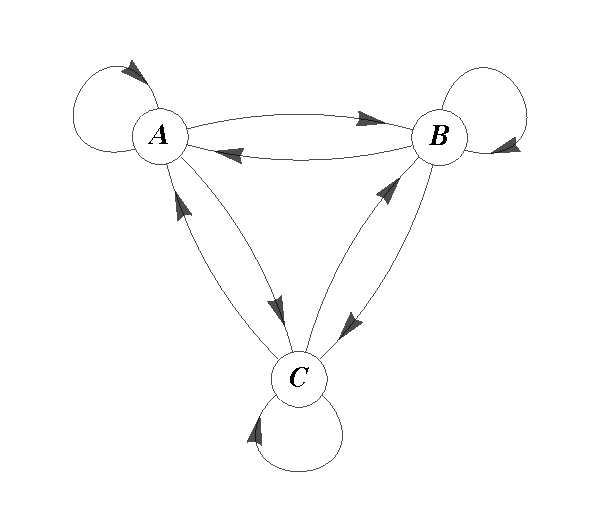
\includegraphics[width=\wid]{figures/K3.pdf}}
\setbox0=\hbox{\hskip -1cm\lower 1.25in\copy0}
\dp0=0pt
\copy0&\multicolumn{1}{c}{\raise 1cm\hbox{$
{}\hskip -2cm\left(\begin{array}{ccc}
1 & 1 & 1 \\
1 & 1 & 1  \\
1 & 1 & 1 \\
\end{array}\right)
$}}\\
&$
{}\hskip -2cm\left(\begin{array}{ccc}
\pair AA & \cdots & \cdots \\
\pair BA & \pair BB & \cdots  \\
\pair CA & ~~~~\pair CB ~~~~& \pair CC \\
\end{array}\right)
$
\end{tabular}
\vskip .2ex
\mycaption{Representations of the complete directed graph $K_3$, where there is an edge $u\rightarrow v$ for each directed pair of the $3$ vertices $u,v \in \{A,B,C\}$. As can be seen (left), the graph is composed from $6$ trivial cycles: 3 are single-arrow cycles (e.g., $\pair AA$), and 3 are double-arrow cycles (e.g., $\pair AB$). The corresponding cycle matrix is shown top right. The cycles represented by it are shown explicitly in the matrix below, which has one entry shown for each trivial cycle. The omitted entries in the matrix are implied by symmetry, as, for example, the top right would be $\pair AC$ but this is the same cycle as $\pair CA$, which is shown bottom left.}
\label{completeg}
\end{center}
\end{figure}

Hence the following algorithm (written in C) is suggested.  The Euler walk is a simple recursive algorithm:
 
%define define-non-randomised-walk /Verbatim/+1, /Verbatim/-1
\begin{Verbatim}
void walk(int u, int v) // follow a cycle starting u -> v
{   recordEdge(u, v); // record the edge walked
    walked[u][v] = walked[v][u] = 1; // keeps the matrix symmetric
    // find all unwalked cycles starting at vertex v
    for( int w = 0; w < N; w++ )
    {   if( !walked[v][w] )
        {   walk(v, w); // start of either a cycle of length 1 or 2
            if( w != v ) // if a cycle of length 2
                walk(w, v); // walk the rest of it
        } 
    }
}
\end{Verbatim}

In this code, vertices are numbered $0$ to $N-1$. \texttt{recordEdge} can be any way of recording the next edge along the Euler cycle; just printing it is easiest:

%define define-basic-recordEdge /Verbatim/+1,/Verbatim/-1
\begin{Verbatim}
void recordEdge(int u, int v) 
{   printf("(%d, %d)\n", u, v); // print an edge walked
}
\end{Verbatim}

The initial call of \texttt{walk} to generate a solution is now simply:  

%define main-body /Verbatim/+1,/Verbatim/-1
\begin{Verbatim}      
walk(0, 0); // walk starting from 0 returning to 0
\end{Verbatim}

Calling \texttt{walk(0, 0)} assumes the sequence always starts and ends at 0. We discuss alternatives in the next section, below, to randomise the cycle and to avoid always starting a cycle on the same edge.

Finally, the \texttt{walked} matrix needs declaring and initialising: 

%define declare-initialise /initialise/, /end{Verbatim/-1
%define declare-walked .+1, .+1
\begin{Verbatim}
int walked[N][N]; // represent a complete graph with N vertices

void initialise() // initialisation; all edges initially unwalked
{  for( int u = 0; u < N; u++ )
      for( int v = 0; v < N; v++ )
         walked[u][v] = 0; 
}
\end{Verbatim}

In C, arrays can easily be initialised to zero when declared, so an explicit initialisation is not strictly required, but we provided explicit initialisation here in case the code is to be translated to another language (or needs to be re-entrant). 

\subsection{Randomised sequences}\label{randomise}

Performing a sequence of experiments in random order controls the effects of drift and random error, and adding the constraint that every calibration value in the set must be preceded exactly once by every other calibration value in the set normalises any carry-over effects. Therefore, for experimental design, we need to modify our algorithm so that the search for an unwalked cycle to recursively follow is randomised. Karl Popper called such sequences ``shortest random-like sequences'' \cite{popper}. The easiest way to do this is to use a random permutation in \texttt{walk}'s \texttt{for}-loop, as follows:

%define define-randomised-walk /verbatim/+1,/verbatim/-1
\begin{verbatim}
void walk(int u, int v) // follow a cycle starting u->v...
{   recordEdge(u, v); // record the edge walked
    walked[u][v] = walked[v][u] = 1; // keeps the matrix symmetric
    // find all unwalked cycles starting at vertex v
    for( int w = 0; w < N; w++ )
    {   int randomisedw = permutation[v][w];
        if( !walked[v][randomisedw] )
        {   walk(v, randomisedw);
            if( randomisedw != v )
                walk(randomisedw, v);
        }
    }
}
\end{verbatim}

Here, \texttt{permutation[v]} provides a randomised permutation of the numbers $0$ to $N-1$, the value of \texttt{w} being mapped by \texttt{permutation[v][w]} to a random value in that range. 
There are $N$ independent permutations (indexed by \texttt{v}) to avoid any dependencies between choices made at each vertex.  Unfortunately, this simple randomisation is not completely uniform, since only the outgoing edge from $v$ is randomised; the return to $v$ always happens last at the randomised vertex. Hence if $u\rightarrow v$ $(u \neq v)$ is the first entrance to $v$, then $v \rightarrow u$ will be the last exit from $v$. For most applications, this is at most a merely technical problem; in particular, because an Euler cycle is a cycle, it can be rotated and started at any point, and this trick can be used to change the ``last'' exits for any vertices.

The Knuth-Fisher-Yates shuffle \cite[p145--146]{knuth2} is a standard way to initialise such a permutation matrix:

%define declare-permutation /int/, /int/
%define initialise-permutation /for/, /end/-1
\begin{verbatim}
int permutation[N][N];
...
for( int u = 0; u < N; u++ )
    {   for( int v = 0; v < N; v++ )
        {   int randomv = randInt(v+1);
            permutation[u][v] = permutation[u][randomv];
            permutation[u][randomv] = v;
        }
    }
\end{verbatim}

To avoid always starting an Euler cycle at the same vertex, the base call \texttt{walk(0, 0)} (which always starts and finishes at 0) must be randomised too:

%define randomised-main-body /verbatim/+1,/verbatim/-1
\begin{verbatim}
randomU = randInt(N);
randomV = randInt(N);
walk(randomU, randomV);
if( randomU != randomV )
    walk(randomV, randomU); // get back to randomU
\end{verbatim}

Since the Knuth-Fisher-Yates shuffle is carefully designed to generate a uniform distribution of permutations, the choices made in the modified \texttt{walk} will be uniformly random. Therefore the series of randomised walks generated by the above code will be uniform samples of all possible Eulerian cycles.

The function \texttt{randInt(N)} provides a uniformly distributed integer from $0$ to $N-1$ inclusive; it is not standard C, but can be approximated from the standard \texttt{rand()} function which produces a pseudo-random integer \texttt{0}..\texttt{RAND\_MAX}. 

%define define-randInt /verbatim/+1,/verbatim/-1
\begin{verbatim}
int randInt(int n) // return random integer 0..n-1 inclusive
{  return floor(n*((double)rand())/((double)RAND_MAX));
}
\end{verbatim}

This code assumes $n<\!\!<\mbox{\tt RAND\_MAX}\approx 2^{31}$ \cite[p119]{knuth2} --- very reasonably, since the length of a Euler cycle is $n^2$, and it is hard to imagine experimenters (even robots) will have the time to perform sequential experiment runs longer than 10,000, which assumption keeps $n\leq100$. 

Finally, note that to ensure different random sequences each time the program is run, the random number generator must be seeded differently during initialisation. This may be done in C from the current time:

%define initialise-Random /verbatim/+1,/verbatim/-1
\begin{verbatim}
time_t t;
srand((unsigned) time(&t)); 
\end{verbatim}

\subsection{Solving the wine tasting problem}
The basic algorithm, described above, uses integers as the names of vertices. For many applications it may be more appropriate to use strings. We can define vertex name strings:\footnote{Not shown here, but our wine sequence generating program, which is generated automatically from this paper using reverse literate programming, checks at run time that \texttt{N} correctly matches the number of wines declared. (It is a shame that this cannot be performed with a static check in C.)}

%define wine-names /verbatim/+1, /verbatim/-1
\begin{verbatim}
// assuming N = 3 (C permits N > 3, which will not work well!)
char *wines[N] = { "Merlot", "Pinotage", "Shiraz" }; 
\end{verbatim}

and then convert the edge recording by changing \texttt{recordEdge} to print the names of the vertices rather than their numbers: 

%define define-wine-recordEdge /Verbatim/+1,/Verbatim/-1
\begin{Verbatim}
void recordEdge(int u, int v) 
{   printf("%s $\\rightarrow$\n", wines[u]); // print the edge walked
}
\end{Verbatim}

\label{winelist}
\ldots\ and finishing with a final \verb|printf("%s\n", wines[0])|, which was otherwise lost in changing the \verb|recordEdge| to only print one vertex rather than pairs. Note how we used \LaTeX's \texttt{\$\char'134rightarrow\$} to generate a ``$\rightarrow$'' symbol to make the experiment sequence look a bit neater when typeset by \LaTeX\@. With these changes, the code generates the following sequence: \input winelist.tex\unskip.

It is easy to confirm by hand that this is indeed an Euler cycle (perhaps by mapping wines to the letters $A,B,C$ and ticking off the edges in figure \ref{completeg}). Note that, as an Eulerian cycle ends at the starting vertex, an additional drink of \input lastwine.tex\unskip\ (in this worked example)\footnote{The wine experiment sequence was generated automatically from the code shown in this paper; it was run and the results saved to a file \texttt{winelist.tex}, the last line of which was extracted (several times) for this paragraph by using Unix's \texttt{tail -n 1 winelist.tex}.} is required: thus a balanced scientific experiment would repeat sequential experiments with randomly selected starting vertices each time, using the ideas of section~\ref{randomise}. Randomisation avoids the potential bias caused by drinking too much \input lastwine.tex\unskip\ --- in the sequence above \input lastwine.tex\unskip\ happens to be drunk both first and last, and hence once more than any other wine. Randomisation also avoids the possible bias caused by always starting with \input lastwine.tex\unskip, which might, for instance, be somebody's favourite wine. After enough randomised sequential experiments, these biases will be evened out.

%An Euler cycle of a complete graph gives us all pairs or 2-tuples of vertices. We note that the generalisation to all sequences of $k$ varieties of wine requires $k$-tipples.

Wine buffs will be tempted to test the algorithm with larger $N$\@. It would certainly be fun to take four varieties of wine to K\"onigsberg (the original graph had $4$ vertices and $7$ edges), cross a bridge, drink the wine variety available on the land, then cross the next bridge, and consider the wine on the other side of the river. As it happens, K\"onigsberg does not have an Euler cycle, so this experiment could take a long time and might result in a new meaning for ``drunken walks.''

\section{Finding algorithms}\label{new-approach}
While we continue to take it for granted that algorithms are described in English, in psuedo-code, with illustrative fragments of uncompilable code, or left as exercises for the reader, unnecessary errors often persist in their real-life implementations. (Some of the problems are reviewed in \cite{heedless,jmlr}.) Often, of course, publications are not always aiming to describe the algorithm as such, but to do something else --- like teach students, analyse complexity, prove some theorems, discuss how to optimise them, and so on. This ``dual use'' creates things that look very much \emph{like\/} algorithms but which cannot be reliably used in practice \emph{as\/} algorithms; the likely confusion calls to mind Feynman's critique of cargo cult science \cite{feynman}. 

Ironically, then, in one of the very few areas --- programming --- where we could be completely explicit about our work (e.g., if an algorithm works, it is text that can surely be published explicitly) there is a default culture of vagueness and ``abstraction'' that undermines scientific reproducibility if not progress. English, pseudo-code, fragments, exercises~\ldots\ none are scientific statements: they are irrefutable \cite{popper}. 

Often software practice and experience emphasises the efficiency of running programs, but we should also be concerned with the end-to-end time to develop a program, confirm it is correctly implemented, and to run it. In many cases, the development time dominates the run time. Unlike the bulk of the algorithms textbook literature, our goal was to have a reliable program quicker, not a faster program later. As we shall argue, literate programming and its variants are powerful approaches to be more scientific when publishing algorithms, and hence to end up with more reliable programs working in the wider world. In this paper, we developed a new variant of literate programming for this very reason.

Programs that can be compiled and run involve details that are generally not relevant to discussions of algorithms. Furthermore, writing a paper or book is a human process, so transcription errors may creep into any algorithms presented. 

There is even the danger that publications may be sloppy: sometimes, authors do not check their published code adequately and referees take the correctness of the code on faith (partly because it is too hard to reconstruct the code from the paper, and too hard to disentangle whether problems are due to the published code or the referee's own errors in the reconstruction of it). ``Sloppy'' is a harsh word, but it covers a wide range of common problems ranging from deliberate fraud, unintentional exagerration, accidental uncorrected errors, and well-intentioned aspirational comments --- like, the program would \emph{obviously\/} work like this (even if it doesn't quite work yet). Even trivial and excusable errors, like typos and spelling errors, undermine the reproducibility of program code.

All this means that finding an algorithm in the literature that can be used to solve a real problem is fraught with difficulties. In our case, having developed an algorithm to solve our problem --- because it is a very common problem for experimenters who may not have sufficient programmering expertise --- we wanted to take care that what we published (i.e., this paper) would be both clear and able to be copied from the paper as real, executable code without problem. We wanted to make it readily --- and reliably --- available.

At the start, we developed and wrote our algorithm first in Mathematica then in C, which is non-proprietary and more portable. Mathematica is excellent for presenting the \emph{results\/} of programs in papers, but it is not good for writing papers \emph{about\/} algorithms, as it requires code to be runnable. In a paper you generally want to discuss fragments of an algorithm in any order that suits the exposition. But because we were excited by our algorithm, we started to write this manuscript, using the very flexible typesetting system \LaTeX\ \cite{latex} to publish and share our findings.

%Originally, we developed a C program (as one does), and then seeing how useful it would be for other people, we decided to write this paper to describe the new algorithm. This paper was then written in \LaTeX, one of many word processing/typesetting systems that are appropriate for writing papers. 
As we wrote, we reviewed and revised the paper. We naturally made many changes to the program code. For example, originally we had used variables \texttt{i}, \texttt{j}\ldots\ in the program, but for writing the paper we decided to use \texttt{u}, \texttt{v}\ldots\ as these are conventional names for graph vertices.\footnote{Unfortunately wines starting with u, v, w, are not commonly recognisable.} So, over time, the original code and its description in the manuscript drifted far apart; yet, in principle, it should have been essential that the manuscript was synchronised with the source code so that it described the source code without error. Ideally, the paper should automatically change to reflect updates to the source code.

In a word, we did not want to be sloppy, yet our initial approach to writing the paper was making life hard. It was tempting to take an easy approach, and only describe our algorithm in words or pseudo-code, being a bit vague about the details. Conventionally, neither the readers of the paper nor we, the authors, would worry about slight discrepancies, because they would be invisible and unknown.

An obvious way to help ensure that executable code transcribed from a manuscript is correct is to cut and paste the relevant text in the paper to reconstruct a new program. However the presence of typesetting commands in \LaTeX\ documents means that the \LaTeX\ code used to generate the manuscript will by necessity differ from the source code of the executable file, so a simple ``cut and paste'' approach is unreliable. But why do something by hand when you can design a tool to do it with far more generality and reliability? Once a tool is written to do this chore automatically, this frees the authors from worrying about maintaining and checking the code in the document as it is repeatedly edited and revised: it should be done automatically.

This idea is very similar to Knuth's \emph{literate programming}~\cite{litprog} which combines source code with explanatory documentation; however the format of the documentation generated by literate programming is not suitable for a journal manuscript. Literate programming also has the disadvantage for us (and for many authors) that the author has to start with the literate program, and in this instance we had already drafted the manuscript as a \LaTeX\ document. \name{Warp\/} is a type of literate programming that extracts code from a normal program commented in XML, thus avoiding the separate processing that literate programming normally requires to generate the executable program \cite{warp}. Our earlier paper in \emph{Software---Practice and Experience\/} on the related Chinese Postman Tour \cite{cpp} used \name{warp\/} to present accurate Java code.\footnote{The Chinese Postman finds the shortest cycle in a graph that is not necessarily Eulerian (i.e., some edges may need to be walked more than once); it is a non-trivial generalisation of the problem discussed in this paper.} \name{Loom\/} \cite{loom} (originally written by Janet Incerpi and Robert Sedgewick for their classic algorithms book \cite{sedgeoriginalbook}) is another approach, similar to \name{warp\/}, but allows the use of Unix filters to perform arbitrary transformations of code (e.g., to handle special symbols) that is then inserted into arbitrary documents. 

In the present paper, however, we had already been working on the code \emph{in\/} the paper, in the usual informal way. To avoid this becoming increasingly sloppy (or, conversely, a huge burden to manage), we therefore developed a novel ``reversed'' literate programming approach: using it, the code is exactly as written in this paper (i.e., what you are now reading) \emph{and\/} it can be automatically extracted to generate a program that is directly executable. The point is: we know that the code shown in this paper works, and moreover, we have a fully automatic process that goes from this paper to executable code. What you now see may not be all of the code,\footnote{There is exactly one line missing; see section \ref{invisible-code}.} but the code shown \emph{does work\/} as shown.  

%there is nothing in the approach that ties it to programs; the method can be used to generate any type of text from a document.) 

Figure \ref{fig:lp} compares the main forms of literate programming, including our new approach. There are of course many other related approaches, ranging from the very simple such as our reverse literate programming to the highly sophisticated, such as Pre\TeX\ \cite{pretex} that are designed for large complex projects and have commensurate learning curves; for a review see \cite{warp}.

\def\mycaption#1{\sf\bfseries\caption{\sf #1}}
\begin{figure}
\begin{center}
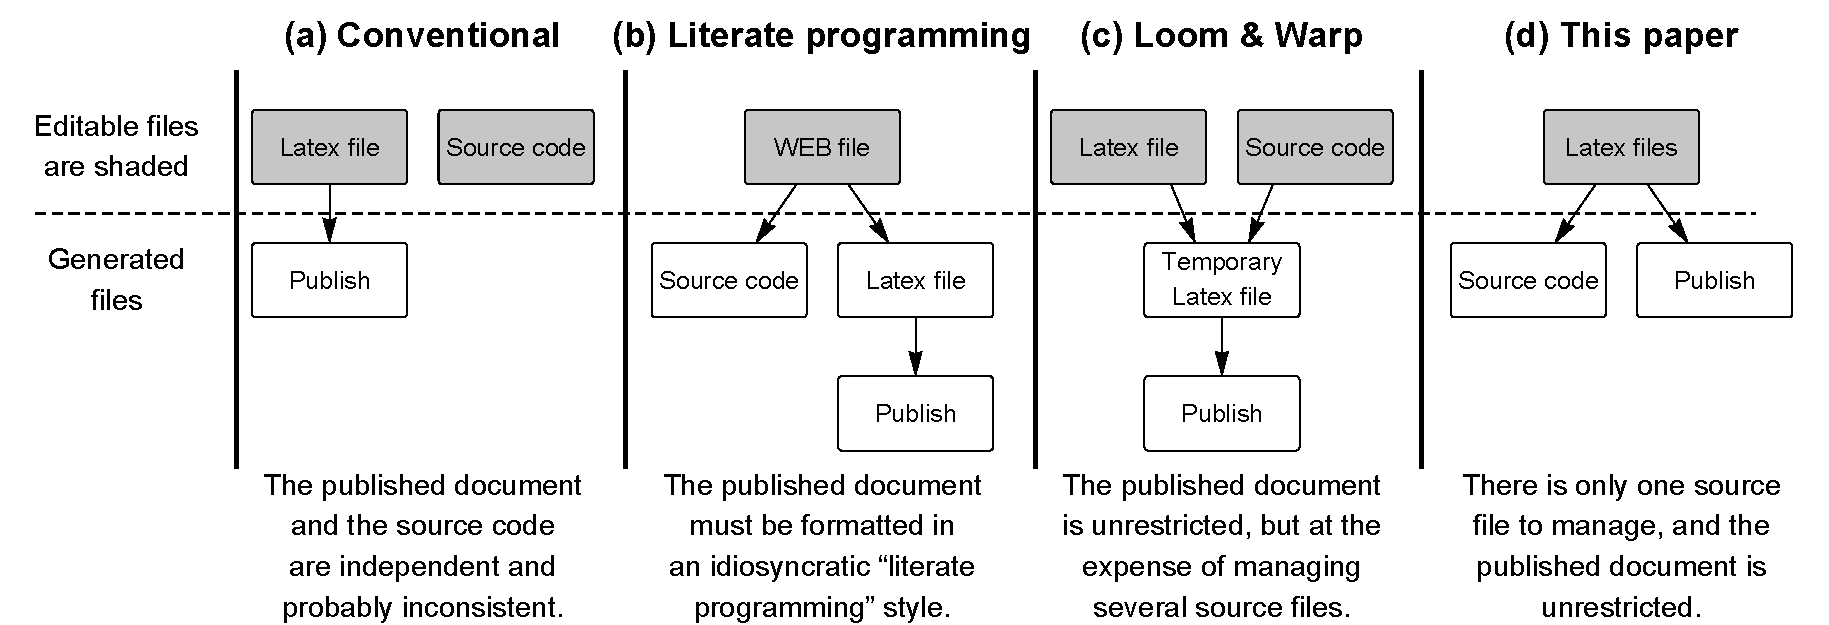
\includegraphics[width=.9\textwidth]{figures/literateProgramming.pdf}
\end{center}
\mycaption{Comparing various ways to write about programming. Note that in the conventional approach (a) there is no guarantee that the published paper faithfully represents the source code, as the paper and source code can be (and will be) edited independently: what is published has no automatic connection to the source code. (Although not made clear in the diagram, typically source code and \LaTeX\ documents will be split into multiple files for convenience. All methods can handle multiple files.)}
\label{fig:lp}
\end{figure}

\subsection{Reverse literate programming --- the details}

Code formatted in this paper is written in the following conventional \LaTeX\ style:

\begin{verse}\tt
\char'134 begin\{verbatim\}\\
printf("Hello world!\char'134n");\\
\char'134 end\{verbatim\}
\end{verse}

There is nothing unusual in this. However, we need to be able to generate a compilable program from such code snippets, even though they may be scattered throughout the paper. In our approach, using our new tool \name{relit}, we name these snippets, and then use the names to generate compilable code.

A name is defined by preceding any part of the \LaTeX\ document with a special comment: 

% the %{} below stops the literate programming thing recognising %{}define!
\begin{verse}\tt
\%{}define \emph{name} /\emph{start pattern}/$\pm$\emph{offset}, /\emph{end pattern}/$\pm$\emph{offset}
\end{verse} 

The pattern style (general regular expressions are permitted) is deliberately reminiscent of the form used by the Unix utility \emph{ed}, and the entire line (starting with the standard \LaTeX\ comment symbol \texttt{\%}) is comment so it is ignored completely by \LaTeX\ itself. 
The effect is that \texttt{\emph{name}} is defined to be the text in the file over the specified range of lines. For example, the code extract above could be preceded with a definition of the name \texttt{demo}:

\manualrelitindex define demo
\begin{verse}\tt % note how we stop the %{}define being recognised
\%{}define demo /verbatim/+1, /verbatim/-1\\
\char'134 begin\{verbatim\}\\
printf("Hello reverse literate programming!\char'134n");\\
\char'134 end\{verbatim\}
\end{verse}

% it's too hard to have a verbatim inside a verbatim, which was needed above, 
% so we now define <demo> so everything works as just described
\def\ignore#1{}
\ignore{
%define demo /verbatim/+1, /verbatim/-1
\begin{verbatim}
printf("Hello world!\n");
\end{verbatim}
}

This defines the name \texttt{demo} to be the text between the two \texttt{verbatim} lines (which are required by \LaTeX\ to typeset the code to see as shown above), namely \texttt{printf("Hello reverse literate programming!\char'134n")}.

A document can generate any number of source code files, by writing analogous file definitions such as:

\begin{verse}\tt
\%{}generate \emph{filename} ., /\%end/-1\\
\emph{text}\ldots\\
\%end
\end{verse}

where within \texttt{\emph{text}} any occurrence of \texttt{<\emph{name}>} is replaced by its definition (and so on recursively). For example,

\manualrelitindex generate hello.c
\begin{quote}\begin{verbatim}
%generate hello.c ., /%end/-1
int main(int argc, const char *argv[])
{ <demo>
  return 0;
}
%end
\end{verbatim}\end{quote}

will generate a file called \texttt{hello.c} that should compile and say hello --- except, of course, compiling it will generate the warning that \texttt{printf} has not been defined. But that is the point: the reverse literate programming enables us to write a paper \emph{and\/} check whether the code we are writing is valid. 

As a matter of fact, we realised we needed to add some explicit code to the paper only after we had implemented reverse literate programming and found some oversights in our original description. Reverse literate programming helped us find the oversight: various declarations and a bit of wider context were needed to make the code described earlier in this paper compile and run without error. The following code generation, creating a file \texttt{euler.c}, works correctly once \name{relit} substitutes the values for the various names, which have been defined elsewhere in this paper:

\manualrelitindex generate euler.c
\begin{quote}\begin{verbatim}
%generate euler.c ., /end/-1
#define N 5 // for a graph with N vertices
<common-declarations>
<declare-walked>
<define-basic-recordEdge>
<define-non-randomised-walk>

int main(int argc, const char *argv[])
{ <main-body>
  return 0;
}
%end
\end{verbatim}\end{quote}

This code was written exactly as shown, and it is easy to check it actually works: it generates the file \texttt{euler.c} which was compiled and run, with the expected results. This implies the code \verb|<main-body>| and so on recursively also compiles and works. Using a makefile (also generated by \name{relit} from the same document) made it very easy to automatically update the code files and unit test them repeatedly as the publication evolved.\footnote{\name{Relit} only updates generated files when their content changes, which makes using \name{make} very efficient, as most edits to a document do not update any files generated from it.}

Of course it is unlikely that a normal paper (that is, one not explaining \name{relit}) would present the code shown explicitly above: usually, the \texttt{\%{}generate} command would have appeared after \LaTeX's \verb|\end{document}| so it would disappear and not be typeset as part of the published paper. Similarly any details that need not be part of a typical published paper can also be hidden. As we will discuss in section~\ref{invisible-code}, \name{relit} can tell the author what code is visible and what code has been hidden to avoid any uncertainties.

Notice that the \name{relit} approach allows the generated program code to be put in the correct order required for a compiler, but the code it is assembled from --- here, \verb|<common-declarations>|, etc --- can be presented to the reader of the paper in any order, in particular in the order that is best for the narrative of the publication. For example, \verb|<main-body>| might be explained to the reader first \emph{then\/} followed by increasing levels of detail of the implementation. Furthermore, if the author decides to rearrange the structure of the paper to improve its exposition this has no effect on the order of the generated code for the compiler.

Similarly, there is no restriction on the order of generating files: they can be specified in any order that best suits the needs of the author.  

Name definitions in \name{relit} can occur before or after they are used; in this paper the definition of the common declarations (standard header files, etc) appears after the end of the \LaTeX\ document and is therefore not typeset anywhere in this paper: the headers are a detail we feel readers of the present paper do not need to see written out in detail, but they are necessary if the paper is to be able to automatically generate executable code. An alternative approach that could be used with C is to only generate ``interesting'' part of the code and use C's \texttt{\#include} from another C file to include the generated code made from \LaTeX\ into a bigger program that provides the correct context to compile and run them.

In general, authors of papers may want arbitrary text generated from programs (for example, we showed the text generated by running our algorithm on a selection of wines), and the generated text may require sophisticated testing. There are many ways to do this: \name{loom} for example, generalises \LaTeX's \texttt{\char'134input} command to allow arbitrary processing, but this has the disadvantage that the approach requires an intermediate \LaTeX\ file to be generated. Instead, our simple approach is to use \texttt{\%{}generate} to create a makefile or any shell script: then any processing whatsoever can be performed, and of course it will typically generate files that are then included in the \LaTeX\ paper. Indeed, this is how we generated the sample list of wine tasting --- using the makefile generated by \name{relit}, Unix's \name{make} then generated a C source program \texttt{wine.c} from the paper you are reading, which was then compiled and run (in the same run of \name{make}), obtaining results saved to a file. Finally, that file was read in at the appropriate point when this paper was typeset (in section \ref{winelist}), using \texttt{\char'134input} to read in the program's saved output to insert it into the paragraph where it was needed. 

The approach is both very general and ensures \emph{everything\/} is kept in one place in a single \LaTeX\ source file, where it is easy to edit reliably. 

Names can also be defined in the tool's command line parameters, so any textual information can be imported when the tool is run --- such as a version number, the date, or even output from \name{expect} to refer to unit test diagnostics. Of course, files created by reverse literate programming can be processed by other tools in arbitrary ways, for example stream editors to decode \LaTeX\ typesetting conventions (e.g., in normal \LaTeX, the common programming symbol \texttt{\&} has to be written \texttt{\char'134\&}).

Our reverse literate programming tool \name{relit} provides all the normal checks, such as reporting if names are defined and never used, used recursively, etc. 
%\name{Relit} also warns if a name is used more than once, since this may indicate an error (if the same piece of code is needed twice in a paper, it probably needs explaining). 
Indeed, some authors have used deliberate ``errors'' as a way of providing metacomments: defining an unused name results in its name and value being reported to the user --- so the text is highlighted, which can be used as a reminder to the author to fix a problem with the document. 

\name{Relit} is a short C program, \input linesofrelit.tex\ lines long.

\subsection{Checking hidden code}\label{invisible-code}
\def\seen{\color{black}\ttfamily\fontseries{l}\selectfont\global\def\endline{}}
\definecolor{highlight-color}{rgb}{1,0.2,0.2}
\def\hidden{\ttfamily\fontseries{b}\selectfont\emph{$\ast\ast\ast$ hidden $\ast\ast\ast$}}
\def\unseen{\color{highlight-color}\ttfamily\fontseries{b}\selectfont\global\def\endline{\hfill~~\hidden}}

The authors of a paper should be able to check that the explicit code shown in their paper is exactly what they want the reader to see and that nothing critical has been omitted. On the other hand, a published paper should conceal details that are distracting or irrelevant to its core message: it need not show all of the code a runnable program requires, but just enough to get the idea across. The tension between these, being explicit and being concise, is a recipe for error: what is hidden, by definition, cannot be seen, yet some omitted information may be required for achieving a complete program. Worse, the reader of the paper may not be certain what is missing, and they may not have the skills or time needed to reconstruct it correctly. Compounding the problem is the so-called ``curse of knowledge'' \cite{pinker}: the authors of the paper have privileged knowledge (in principle they know everything about what they are talking about) and they may therefore be unaware that some things have not been explicitly mentioned in the paper --- it is very hard to distinguish between what they know in general about what they are writing and what they think they know (perhaps inaccurately) is in the paper.

Tools like \name{warp} and \name{loom} help the authors ensure that code published has been obtained directly the working programs, but it is still possible to write code in the paper that has never been tested or compiled, and also to leave a lot of essential context in the program that \name{warp} or \name{loom} do not draw into the document. Figure \ref{fig:lp2} summarises the issues. 

\begin{figure}
\begin{center}\sf\small
\def\ast{\hskip 0.1pt{\lower .5ex\hbox{\large$\star$}\vphantom{\Large y}}}
\newdimen\cola \setbox0=\hbox{programming} \cola=\wd0 \advance\cola by .5em
\newdimen\colc \setbox0=\hbox{diagnostics} \colc=\wd0 \advance\colc by .5em
\def\gap{\vskip .5ex\hrule\vskip .5ex}
%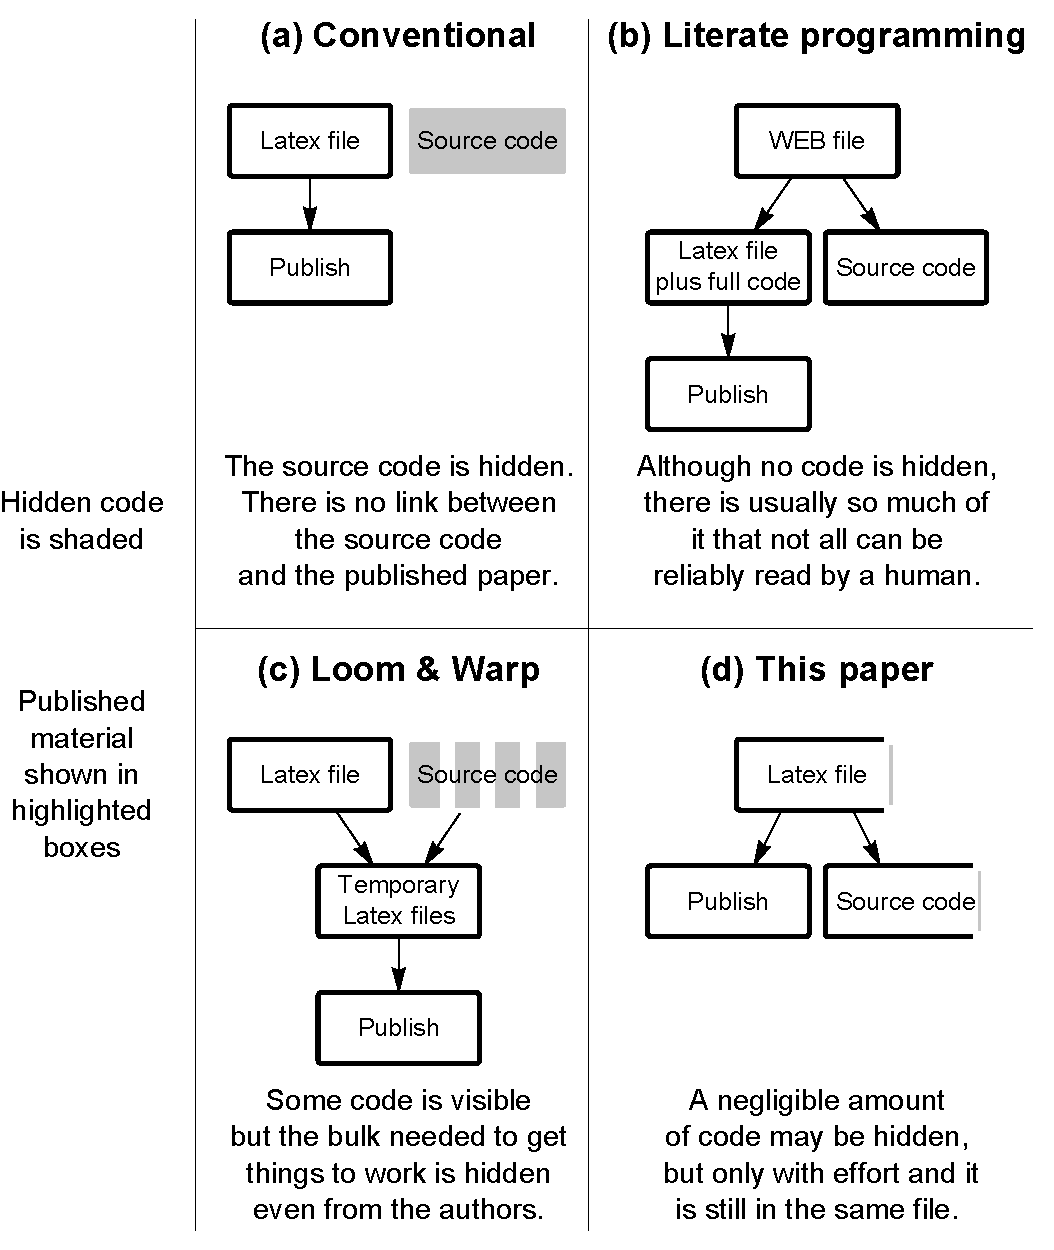
\includegraphics[width=.9\textwidth]{figures/hiddenCode.pdf}
\noindent\begin{tabular}{|p{\cola}|p{3.4in}|p{\colc}|}  \hline
\bfseries Reverse literate \hbox{programming}& 
A negligible amount of code may be hidden, but only with deliberate effort. All code remains in the same file --- so it is easy to see and edit without introducing errors. Negligible learning curve; no extra steps. Intended for peer reviewed publications. &\hfil\ast\ast\ast\ast\hfil \gap Typically only one file to maintain. \\ \hline

\bfseries \hbox{Loom} \hbox{and Warp}& 
Some code is visible, but most is hidden --- it remains in separate code files. Small learning curve; extra step needed in writing process. Good for publications.&
\hfil\ast\ast\ast\hfil  \gap Any number of files. \\ \hline

\bfseries Literate \hbox{programming}& 
No code is hidden and all the code and document is in one place, but there is usually so much code that not all can be reliably read by a human.  Steep learning curve; extra steps needed in writing and compiling processes. Ideal for internal documentation rather than peer reviewed publications.&
\hfil\ast\ast\hfil \gap Typically few files to maintain.\\ \hline

\bfseries Conventional approach& 
Source code is hidden. There is no link between the source code and the published paper. Errors and inconsistencies are easy to introduce. No learning curve.&
\hfil\ast\hfil \gap Any number of files. \\ \hline

\end{tabular}

\vskip .5cm
\begin{tabular}{cp{4.75in}}
\ast\ast\ast\ast & All source code and published paper in a single document. \par Diagnostics for both missing and defined but unused code. \par Flexible indexing, in published document and in command line. \\ \hline
\ast\ast\ast & Some source code is published. \par Diagnostics for missing code, but some code can be defined (i.e., intended for use) but accidentally left unused. \par No indexing. \\ \hline
\ast\ast & All source code is published. \par No diagnostics necessary. \par Sophisticated indexing in published document. \\ \hline
\ast & No connection between published paper and program source code.\par No diagnostics possible. \par No indexing. \\ 
\end{tabular}
\end{center}
\mycaption{The more code that is hidden, the more likely it will drift into complexity and concealed critical details. Conventional literate programming hides nothing, but typically makes the result too large to be publishable (\name{JavaDoc} only documents the API rather than the entire program). \name{Loom} and \name{Warp} help ensure code published is correct, but it may be incomplete. The present paper's reverse approach, as embodied by \name{relit}, ensures almost all the code is published, and what the authors may choose not to publish can easily be checked with simple diagnostics (see section~\ref{complete-program}) --- and what is not published remains in the original \LaTeX\ files, so the authors always remain aware of it.}
\label{fig:lp2}
\end{figure}

Unfortunately, in reverse literate programming, since generated code can include names that are defined anywhere in the documents, and the defined values themselves may or may not be visible in the published paper, and so on recursively, it is impractical to manually determine what code is visible in the published paper and what, if any, is not visible.

Our reverse literate programming tool, \name{relit}, allows code to be tagged, and although the tags can be used for any purpose, a useful application is to keep track of what code is visible and what is not. The approach is simple; the \texttt{define} and \texttt{generate} commands can be followed by optional tags:

\begin{verse}\tt
\%{}define \emph{name} \emph{start}, \emph{end} [, \emph{tag}] \\
\%{}generate \emph{filename} \emph{start}, \emph{end} [, \emph{tag}]
\end{verse} 

For every file generated, \name{relit} additionally generates a duplicate file but marked up with the tags, with the relevant tags output as each \texttt{\emph{name}} (or file) is expanded. The tags are arbitrary text, but will typically be \LaTeX\ macro names that can be defined to highlight text. Of course if the tags include names like \texttt{<\emph{name}>} then they will be expanded as normal (the names can be defined anywhere, generally after the end of the document). This feature is useful if the tag is complicated (e.g., writing \texttt{<tag>} is easier and more reliable than writing out a tag in full every time it is needed) or if the author wants a tag to have several lines of text.

With tagging, we can readily obtain typeset text showing where code has come from. 

However, since tagging each \texttt{\emph{name}} definition is a bit tedious --- and therefore itself error-prone --- a default tag can be defined:

\begin{verse}\tt
\%{}set-tag \emph{tag} \\
\end{verse}

That \texttt{\emph{tag}} is then automatically applied to all subsequent definitions (and files) until it is superceded, or overridden by explicit tags. Hence, typically a \LaTeX\ document will start:

\begin{verse}\tt
\ldots \\
\char'134begin\{document\}\\
\%{}set-tag \char'134seen\{\} \\
\ldots \\
\emph{published document including visible definitions}
\end{verse}

and then have the following at its end:

\begin{verse}\tt
\ldots\\
\char'134end\{document\} \\
\%{}set-tag \char'134unseen\{\} \\
\ldots\\
\emph{hidden definitions and files}
\end{verse}

Here, the \LaTeX\ code \texttt{\char'134end\{document\}} signals the end of the published \LaTeX\ document, and all subsequent text will be hidden from view in the published document. Normally this part of a \LaTeX\ document is empty, or has accummulated ``junk'' text and thoughts the authors cannot steal themselves to \emph{really\/} delete --- the space has a useful role in co-authored documents, where one author wants to delete text from the published document, but does not want another author to lose some idea without a chance to reconsider it before it is deleted. In our case, with reverse literate programming, the hidden space can also be used for defining program code that is needed for compiling and testing, but is considered too much detail for visible inclusion in the published document.

The illustrative tags \texttt{\char'134seen\{\}} and \texttt{\char'134unseen\{\}} used above are arbitrary; one might choose to use \texttt{\char'134color\{black\}} and \texttt{\char'134color\{red\}} instead, say. In the complete example shown below (having defined \texttt{\char'134unseen\{\}} appropriately)  the ``{\hidden}'' marker is provided automatically and therefore correctly.\footnote{Correctness here depends on the author not cheating! \LaTeX\ is programmable, so a determined author could defeat the reliability of the tagging mechanism if they were so inclined.}

The code shown next, below, is one of the example algorithms as already discussed in this paper: the highlighted text generated by \name{relit} reveals code that was not previously shown in the paper but which was generated for the compiled test programs. In other words, the highlighted code is included in this document, but it was hidden from sight from readers of this paper by being placed after \texttt{\char'134end\{document\}}. 

The authors of this paper are happy that these standard declarations are not taking up space in the published paper --- in any case, if a reader of this paper faithfully copies the published code and omits these lines, good compilers will provide helpful error messages such as ``Note: include the header \texttt{<stdio.h>} or explicitly provide a declaration for \texttt{printf}.''

{\label{complete-program}\tt \vskip .3cm \begin{verse}\small
\input e.txt
\end{verse}
}

To summarise: using this feature of \name{relit} we can assure ourselves that readers of this paper have the complete algorithm to reproduce exactly or as exactly as we want. The one line, highlighted above in the diagnostic output from \name{relit}, shows that in fact our paper does not disclose one line of code. However we consider this omission obvious, unnecessary and distracting implementation detail for the paper. 

Apart from the original literate programming approach that tells the reader everything, which may be overwhelming, we know of no other approach that give the benefits of concise algorithm publication combined with such assurances of reproducibility.

\subsection{A more flexible \TeX-mode}
As described above, \name{relit} uses \texttt{\%} to introduce commands, like \texttt{generate} and \texttt{define}; the advantage of this approach is that \LaTeX\ completely ignores \name{relit} commands because they are in the form of \LaTeX\ comments. However, in addition, \name{relit} provides a ``\TeX-mode'' that makes the syntax it uses real \TeX\ or \LaTeX\ code; this is more sophisticated, requires a little \TeX\ programming, but has advantages that some authors may appreciate.

\begin{figure}
\begin{center}\tt\small\begin{tabular}{ll}
\rm\bf Normal mode&\rm\bf \TeX-mode \\ \hline
\% de{}fine \emph{name} $\mbox{\tt \emph{re}}_1$, $\mbox{\tt \emph{re}}_2$ & \char'134relit\{define \emph{name} $\mbox{\tt \emph{re}}_1$, $\mbox{\tt \emph{re}}_2$\} \\
\% de{}fine \emph{name} $\mbox{\tt \emph{re}}_1$, $\mbox{\tt \emph{re}}_2$, \emph{tag} & \char'134relit[\emph{tag}]\{define \emph{name} $\mbox{\tt \emph{re}}_1$, $\mbox{\tt \emph{re}}_2$\} \\
\% gen{}erate \emph{name} $\mbox{\tt \emph{re}}_1$, $\mbox{\tt \emph{re}}_2$ & \char'134relit\{generate \emph{name} $\mbox{\tt \emph{re}}_1$, $\mbox{\tt \emph{re}}_2$\} \\
\% gener{}ate \emph{name} $\mbox{\tt \emph{re}}_1$, $\mbox{\tt \emph{re}}_2$, \emph{tag} & \char'134relit[\emph{tag}]\{generate \emph{name} $\mbox{\tt \emph{re}}_1$, $\mbox{\tt \emph{re}}_2$\} \\
\% se{}t-tag \emph{tag} & \char'134relit\{set-tag \emph{tag}\} \\
\% \emph{any comments permitted\/} & \char'134relit\{ends\} \\
\end{tabular}\end{center}
\mycaption{Corresponding normal and \TeX-mode \name{relit} syntaxes.} 
\label{fig:syntax}
\end{figure}

Comments get completely lost to \LaTeX, which makes the basic use of \name{relit} easy to understand. On the other hand, an author may wish to see exactly where the \name{relit} commands are and what they do. In \name{relit}'s \TeX-mode, therefore, commands are written as proper \TeX\ commands. Normally, \TeX\ has to define the commands to be ignored, if we want \name{relit}'s behaviour to be exactly as described at length above. However, \TeX\ can also be used to define the commands to do anything, such as printing where they are used in the document to help the authors prepare the paper. \TeX\ can also construct an index of \name{relit} names, as shown in figure~\ref{fig:index}, which may help in large authoring projects.

The \TeX-mode syntax corresponds directly to the original syntax, and is summarised in figure~\ref{fig:syntax}. The final case in the table allows the author to use \texttt{\char'134relit\{ends\}} to match in $\mbox{\tt \emph{re}}_2$ to mark the end of definitions (normally anything convenient, such as text in a comment, can be used). See below for an example of its use.


\name{Relit} warns if \TeX-mode and non-\TeX-mode commands are mixed in the same files: the point of \TeX-mode is that authors can use \TeX\ to keep track of \emph{all\/} \name{relit} commands, but using the \texttt{\%} \name{relit} notation as well (which of course \TeX\ completely ignores) would undermine reliable tracking.

\relit[\seen{}]{generate TeX-mode-demo.tex /indent/, /relit.ends/-1}\label{tex-mode-example}
\indent This and the next paragraph together make up a simple example that generates a file \texttt{TeX-mode-demo.tex} that will contain this text after \name{relit} is run. 

Although normally ignored by \LaTeX\ and invisible to readers, the \name{relit} commands used to save these two paragraphs have been made clearly visible by defining {\tt \char'134relit} appropriately in \LaTeX, as can be seen highlighted on the two lines just before and just after the paragraphs.
\relit{ends}

Notice in this example how we have defined \texttt{{\char'134}relit} so it typesets its parameters to appear directly in the typeset document; this approach can be very useful for helping rewriting and refactoring. The \texttt{{\char'134}relit} definitions used in this paper are readily available: in the same way that \name{relit} is run on this paper to generate compilable programs, an additional \texttt{\%{}generate} command saved the actual definition of \texttt{{\char'134}relit} used above to a file so it can be reused in other documents.

The reason that \name{relit} makes \TeX-mode an option, rather than being the only method of use, is that the feature introduces a conceptual layer of complexity the standard approach does not require. Using \TeX-mode requires not just defining some \TeX\ commands (a matter of copying them from somewhere that already works) but also understanding how to balance \TeX's syntax with regular expressions, which is harder as you can no longer use {\tt \char'134}, {\tt \%}, \{, \}, etc, in the same way. 

{\def\thefootnote{\lower 1ex\hbox{*}}
\setbox0=\hbox{\footnotemark\relax}
\begin{figure}
\renewenvironment{theindex}{\begin{list}{\relax}{}\item \hskip0pt \vdots}{\item \hskip0pt \vdots\end{list}}
\begin{center}\small
\input eulerPaper.ind
\end{center}
\mycaption{A simple \TeX-mode index. For illustration purposes, only names and files explicitly defined in this paper have been shown (this simplified index excludes definitions where the normal \name{relit} process does not show names to the reader, including all other hidden material after the {\tt \char'134end\{document\}}).\copy0}
\label{fig:index}
\end{figure}
\footnotetext{This paper, which is both a paper explaining an algorithm in the usual way and a paper explaining \name{relit} in detail, is complicated by unusually having to write \name{relit} commands \emph{inside\/} \LaTeX\ \texttt{verbatim} environments, so the reader can see them but where simultaneous indexing is impossible. (In normal use, \name{relit} commands would be outside \texttt{verbatim} and similar commands and hence they would be processed by \LaTeX\ and would normally be invisible to the reader.) Thus, index entries marked~* in figure~\ref{fig:index} were provided by using duplicated \name{relit} commands written just outside the \texttt{verbatim} environments so \LaTeX\ could evaluate them to make the starred index entries as shown.}
}

\section{The benefits of automatic honesty}\label{benefits}
\def\startquote{\sf\raggedright\setbox0=\hbox{``}\hskip -\wd0 \copy0}
\def\quoteend{''}

Richard Feynman's opening sentence for his 1965 Physics Nobel Prize lecture~\cite{feynmanprize} (shared with Sin-Itiro Tomonaga and Julian Schwinger) is

\begin{quote}\startquote We have a habit in writing articles published in scientific journals to make the work as finished as possible, to cover all the tracks, to not worry about the blind alleys or to describe how you had the wrong idea first, and so on.\quoteend
\end{quote} 

Here Feynman recalls the common habit we are also prone to in Computer Science when writing articles about algorithms (and when using other formal languages). As we refine and improve our articles, their connection with the orginal programs becomes tenuous. We ourselves encountered this problem in very early drafts of this paper before we had invented \name{relit}: improving the paper led us to talk about variables $u,v$ yet the program we were writing about really had variables $i,j$. The original programs had many details, including essential declarations, that never made it into the working paper. It is too easy to slip from clarifying your writing to simply making it up.

There is a legitimate stage in drafting papers where authors can freely write about what they hope and intend will be true as placeholders for future work. ``Our program \emph{will\/} work like this~\ldots'' But if what they write has no rigorous connection with reality it will never be straightforward to know when the aspirational gap has been closed, and the authors thus risk eventually publishing misleading and time-wasting papers. Readers generally have no way to distinguish sketches and visionary ideas from actual achievements. 

Feynman \cite{feynman} later warned about the utter honesty essential to do good science. In 1974 he said, 

\begin{quote}\startquote 
It's a kind of scientific integrity, a principle of scientific thought that corresponds to a kind of utter honesty --- a kind of leaning over backwards.~[\ldots] In summary, the idea is to try to give all of the information to help others to judge the value of your contribution; not just the information that leads to judgment in one particular direction or another.\quoteend
\end{quote} 

But with computers we can go further than physicists: we can help make honesty automatic. This is so important: when honesty is automatic, it is easy \emph{and reliable}. As Feynman said, 

\begin{quote}\startquote 
The first principle is that you must not fool yourself --- and you are the easiest person to fool.  So you have to be very careful about that.  After you've not fooled yourself, it's easy not to fool other scientists.  You just have to be honest in a conventional way after that.\quoteend
\end{quote}

So automatic tools and techniques to encourage reproducibility, like \name{relit}, can help you help yourself --- and help your readers. Your readers should not have to work out things for themselves you did not know you were not telling them. Our scientific writing should not rely on readers having to use their insight to interpret and clarify what we write; different readers may have different insights, and then it is not clear what our science is communicating.

When describing something that is complicated, there is a temptation to simplify and take short cuts. In the worst case, this results in publications that describe what ought to happen, what we hope happens, but there are omissions that mean the claims are not easily reproducible. Somehow it is too easy to reframe our programs so that it sounds as if they work; all the details are too hard to check even for the original authors --- and as we convince themselves what we write is correct, then there seems to be less and less need to go to the trouble of checking our code. When we conceal errors --- and, worse, when we conceal errors from ourselves --- although our work may look good, it holds back progress \cite{blackbox}.

If a tool like \name{relit} is used, the code in the paper is exactly what works. If describing it gets complicated, this cannot be denied. Instead of simplifying the narrative, the author is encouraged to improve the code so it becomes easier to describe. This means \emph{both\/} the code and the paper improve, and together.

It must be pointed out that not everybody agrees under all circumstances. For example, Knuth writes~\cite[p\emph{vii}]{texbook}:

\begin{quote}\startquote 
The author feels that this technique of deliberate lying will actually make it easier for you to learn the ideas. Once you understand a simple but false rule, it will not be hard to supplement that rule with its exceptions.\quoteend
\end{quote}

His argument is that a reader learns, and at first things need to be simplified with ``white lies'' as he calls them \cite[p44]{texbook}, and then, later with more knowledge and skill, the reader can learn from more elaborate explanations that would have been incomprehensible earlier. However, this is Knuth's strategy for writing his substantial and very successful \emph{\TeX book}, which describes in a single document a very complex system, namely \TeX\ itself. He knows readers will have an arduous process ahead of them, and the book tries to fit the needs of both beginners and experts. We believe that in contrast, in normal scientific publishing, particularly in publishing comparatively short peer reviewed papers --- which normally focus on one or two ideas --- the utter honesty championed by Feynman has important if not overriding advantages. Another point of view is that perhaps Knuth should have improved \TeX\ so it did not require lying to explain it so well. On the other hand, one of the enormous strengths of \TeX\ is that it has \emph{not\/} ``improved'' over time, so it is remarkably portable and dependable, unlike many programs that are continually ``improving'' with new changes forcing users to upgrade.

While the \emph{\TeX book} is an exceptional piece of writing, elsewhere Knuth himself has said science is what we can explain well enough to computers~\cite{a=b}, and that everything else is art. 

Our position is that if people are publishing scientific papers about algorithms that cannot ``be explained to computers'' --- they surely ought to work as described --- then their papers are too obscure to be called science. They are compromising reproducibility. Science advances when art becomes science; we hope, then, that ideas like reverse literate programming will help move the darker arts of publishing programming into an improving science of programming.

\section{Conclusions}\label{conclusions}
We developed a neat algorithm to help perform reliable sequential experiments, and in the process of writing about it clearly we also developed a tool to help publish reliable papers about algorithms. This paper combined a description of the algorithm and a description of the tool that enabled us to write this paper.

Our algorithm generates Euler cycles or randomised Euler cycles for complete directed graphs. It can be used to generate randomised $(N,2)$ de Bruijn sequences for efficient sequential experimental design which controls for random variation, systematic error, and carry-over effects. The simplicity of our algorithm, written in basic C, means that it is easy to understand and translate into other languages, which makes it accessible to those engaged in research. 

Conventional literate programming prevents transcription errors by linking source code and manuscripts. Our novel ``reverse literate programming'' approach, which we have described and used in the preparation of the present paper, has allowed us to simultaneously edit the program code and description in the paper at will, and repeatedly automatically generate an executable program we could then run and use to confirm the integrity of the code we described in the paper. 

Here is one example benefit from our approach. At the last moment, our colleague Paul Cairns pointed out that we had confused wine regions (e.g., Chianti) for grape varieties (e.g., Pinotage and Merlot). In the conventional approach to writing about algorithms, we would have edited the paper and the paper and the programs we had written about would have diverged, or at least we would have needed to edit a variety of files that would then have required tedious manual cross-checking (if we could be bothered to do it). We might have decided it was not worth the bother. We might have fooled ourselves: the program works even if it might get the names of the wine regions or grapes mixed up. Certainly, explaining what needs doing is easier than doing it, and it is then but a short step to justifying to ourselves not doing it because it is easier imagined than done.

Instead, because we were using \name{relit}, we did \emph{one very trivial\/} global edit \emph{in a single file\/} which immediately replaced all our original dubious uses of the word Chianti with Shiraz. This was a trivial change. With no further effort, thanks to using \name{relit}, we automatically had a new C program that used Shiraz, and the output from running it was then automatically inserted back into this paper so the example output (used in section~\ref{winelist}) was also updated to say Shiraz instead of Chianti. Everything remained consistent with no effort. And everything is obviously consistent with the code shown in the paper because it was generated by running exactly the code in the paper that you are reading. Doing it is easier than explaining it.

This paper and the \name{relit} tool and documentation are available from \url{https://github.com/haroldthimbleby/relit}

%The reason for literate programming (reverse or not) is that people want to talk and write about programs in a different way from how compilers need them. There are various automated schemes (such as \name{loom\/} and  \name{warp\/}) and this paper's new approach that make writing \emph{reliably\/} about programs much easier. 

%One can write a paper for human readers, edit the program code in the paper at will, and \emph{then\/} automatically generate a program test bed to check and run the code.

\section*{Acknowledgements}
This research was funded by EPSRC grant no.~[EP/L019272/1]. We are very grateful to Paul Cairns for making us greatly improve the paper.

\let\oldbibitem=\bibitem
\def\bibitem{\frenchspacing\raggedright\oldbibitem}
\bibliographystyle{plain}
\bibliography{eulerPaper}

\long\def\ignore{\begin{thebibliography}{00}
\raggedright

\bibitem{sedgewickcode}
Sedgewick R., Wayne K. \& Liu N., http://algs4.cs.princeton.edu/42digraph/DirectedEulerianCycle.java, 2015.
Cited in Sedgewick R. \& Wayne K., Algorithms, 4th Edition, Addison-Wesley, 2011.

\bibitem{euler}
Euler L. Solutio problematis ad geometriam situs pertinentis. Comment. Academiae Sci. I. Petropolitanae 1736; \textbf{8}:128--140.

\bibitem{wilson}
Hopkins B, Wilson RJ. The Truth about K\"onigsberg. The College Mathematics Journal 2004; \textbf{35}(3):198--207.

\bibitem{cpp}
Thimbleby, H. The Directed Chinese Postman Problem, Software --- Practice {\&} Experience 2003:  \textbf{33}(11):1081--1096. DOI: 10.1002/spe.540

\bibitem{debruijn}
de Bruijn NG. A Combinatorial Problem. Koninklijke Nederlandse Akademie v. Wetenschappen 1946; \textbf{49}:758--764.

\bibitem{fleury}
Fleury, M. Deux probl\`emes de G\'eom\'etrie de situation. Journal de math\'ematiques \'el\'ementaires 1883; 2nd ser. (in French) \textbf{2}:257--261.

%\bibitem{derivere}
%de Rivere, A. (1894) Journal l'Interm\'ediaire des Math\'ematiciens (** FULL REF REQUIRED **)

\bibitem{sainte-marie}
Sainte-Marie CF. Solution to problem number 48. l'Interm\'ediaire des Math\'ematiciens 1894:107--110.

\bibitem{hall}
Hall RW. `Math for Poets and Drummers' \url{http://people.sju.edu/~rhall/mathforpoets.pdf} [25 November 2015].

\bibitem{knuth4a}
Knuth DE. The art of computer programming. Volume 4A\@. Combinatorial Algorithms, Part 1, Addison-Wesley: Reading MA, 1998.

\bibitem{diaconis}
Diaconis P, Graham R. Magical Mathematics: The mathematical ideas that animate great magic tricks. Princeton University Press: Princeton NJ, 2012.

%%\bibitem{livescribe}
%%\url{http://www.livescribe.com} [25 November 2015].

\bibitem{hierholzer}
Hierholzer, C. Ueber die M\"oglichkeit, einen Linienzug ohne Wiederholung und ohne Unterbrechung zu umfahren. Mathematische Annalen 1873; \textbf{6}(1):30--32. DOI: 10.1007/BF01442866.

%\bibitem{lempel}
%Lempel A. On a Homomorphism of the de Bruijn Graph and its Applications to the Design of Feedback Shift Registers. IEEE Transactions 1970. \textbf{C-19}(12):1204--1209. DOI: 10.1109/T-C.1970.222859.

\bibitem{good}
Good IJ. Normal recurring decimals, J. London Math. Soc. 1946: \textbf{s1-21}(3):167--169. DOI: 10.1112/jlms/s1-21.3.167

\bibitem{turan}
Turan MS. Evolutionary Construction of de Bruijn Sequences. AI Sec'11. Proceedings of the 4th ACM Workshop on Security and Artificial Intelligence 2012: 81--86. DOI: 10.1145/2046684.2046696.

\bibitem{fisher}
Fisher RA. Statistical Methods for Research Workers. Oliver and Boyd: London, 1925; 224--233.

\bibitem{aguirre}
Aguirre GK., Mattar MG, Magis-Weinberg L. de Bruijn cycles for neural decoding. Neuroimage 2011: \textbf{56}(3):1293--1300. DOI: 10.1016/j.neuroimage.2011.02.005

%\bibitem{golomb}
%Golomb SW. Shift Register Sequences. Holden-Day: San Francisco CA, 1967.

\bibitem{graphbook}
Chartrand G, Lesniak L. Graphs \& Digraphs (3rd. ed.). Chapman \& Hall: London, 1996.

\bibitem{popper}
Popper KR. The Logic of Scientific Discovery. Routledge Classics: London, 2002.

\bibitem{knuth2}
Knuth DE. Seminumerical algorithms. The Art of Computer Programming, \textbf{2}, (3rd ed.). Addison-Wesley: Boston MA, 1998.

\bibitem{litprog}
Knuth DE. Literate Programming, Center for the Study of Language and Information --- Lecture Notes \textbf{27}, Stanford University, 1992. DOI: 10.1093/comjnl/27.2.97

\bibitem{warp} 
Thimbleby H. Explaining Code for Publication, \emph{Software --- Practice {\&} Experience}, 2003: \textbf{33}(10):975--1001. DOI: 10.1002/spe.537.

\bibitem{loom}
Hanson DR. Printing common words. Communications of the ACM 1987: \textbf{30}(7):594--598.

\bibitem{pretex}
Kruse RL. Managing large projects with Pre\TeX: A preprocessor for \TeX. \TeX\ Users Group Annual Meeting, 1070--1074, 1999.

\bibitem{sedge}
Sedgewick R. Algorithms. Addison-Wesley: Reading MA, 1983.

\end{thebibliography}}
\end{document}
\appendix 
\section{Brief correctness argument}
If a directed graph $G$ is complete, then for all vertices $u,v \in G$\/:

\begin{description}\raggedright
\item[$u\neq v$]:
there is an edge $u \rightarrow v$ for every pair of $u,v$ and there is also an edge $v \rightarrow u$. The pair of edges $u \rightarrow v$ and $v \rightarrow u$ form a trivial cycle, namely $\pair uv$. 
 
\item[$u=v$]: there is an edge $\pair uu$ which forms a trivial cycle. 
\end{description}
 
The initialised cycle matrix therefore correctly represents a complete graph as a composition of trivial cycles. Moreover the matrix is symmetric.

There are many equivalent characterisations of graphs with Eulerian cycles. We use the following: a directed graph has an Eulerian cycle if and only if: (\emph{i\/}) it is strongly connected, and (\emph{ii\/}) it can be decomposed into edge-disjoint (non-overlapping) directed cycles (i.e., each edge is part of exactly one cycle). A proof uses Veblen's Theorem \cite{graphbook}.

As \texttt{walk} recursively expands trivial cycles, it effectively composes the initial decomposition into trivial cycles into an Euler cycle. Therefore the algorithm will print a cycle. Because of the \texttt{walked} test, no edge is walked more than once. The next part of the proof shows that when the walk terminates there are no missed cycles.

After walking an edge, $u \rightarrow v$, in each iteration of the \texttt{for} loop, the body of walk recursively explores every connected vertex from $v$. If we assume no cycles have been walked, then because the graph is complete, every other vertex $w$ will be visited and hence all cycles starting with each vertex will be explored. Hence, the very first call of \texttt{walk} is sufficient to walk every cycle.

Provided the graph remains strongly connected, deleting trivial cycles from the cycle matrix makes no difference to the argument for correct termination. In particular, the algorithm will work correctly regardless of self-cycles $\pair uu$; the graph need not be reflexive, and thus it can find Euler cycles of irreflexive complete graphs.

%A complete graph relates every vertex with every other, and therefore represents an equivalence relation. Graphs represented by the cycle matrix are symmetric relations: if $u$ is related to $v$, then $v$ must be related to $u$ --- hence there exists a cycle $\pair uv$. The cycle matrix diagonal permits reflexive relations, but it does not require them. For example, for integers, the graph of the relation ``$uv$ is even'' is symmetric but only partially reflexive (cases when $u=v$) when $u$ is even.

%The algorithm prints the Euler cycle for a complete graph of size $N$. If the graph is not complete, the initialisation can ``pretend'' missing cycles have already been walked by setting \texttt{walked} to \texttt{1} for the appropriate cycles. However, the cycle matrix representation means that only symmetric graphs can be represented: that is, whenever there is an edge $u\rightarrow v$ there must also be an edge $v\rightarrow u$ (of course, $u\rightarrow u$ is a special case). 

%Not all symmetric graphs are Eulerian and not all Eulerian graphs are symmetric, in which case \texttt{walk} cannot in any case generate an Eulerian cycle --- however, note that it will terminate regardless. In general, a Chinese Postman Tour will find a cycle in any connected graph (possibly walking some edges more than once), and in the special case that the graph is Eulerian, the Chinese Postman Tour will in fact be an Eulerian cycle \cite{cpp} .

%A check that no entries in the \texttt{walked} matrix remain false is sufficient to check whether the graph was Eulerian. The more general de Bruijn sequences $(N,n),~n>2$, which generate all $n$-tuples in order can also be efficiently generated from Euler cycles, but the underlying de Bruijn graphs are not representable as simple cycles, and therefore our algorithm is not directly applicable for $n>2$.

%Of course, the initial call to \texttt{walk} must be on an unwalked cycle, and the graph must be connected for the walk to be able to cover all cycles. Inserting an assertion on line 10 may be advised: \texttt{assert(!walked[u][v])} because line 22 may invoke \texttt{walked} on an impossible path.

\end{document}
%set-tag \unseen{}
\newpage
\color{blue}
\section{Probably obsolete stuff}
\subsection{Final details}
The C code above represents vertices with the integers $0$ to $N-1$. It is easy to convert these numbers to string labels (or any other types) by defining a pointer to a string array, for example:

\begin{verbatim}
char *labels[] = { "A", "B", "C" }; // assuming N=3
\end{verbatim}

and changing line 10 to, e.g., 

\begin{verbatim}
printf("(%s, %s)\n", labels[u], labels[v]);
\end{verbatim}

Finally, correct implementation of this algorithm in C requires \verb|rand()|, \verb|srand()|, \verb|RAND_MAX|, \verb|time_t|, \verb|time()| and \verb|printf()|. Their declarations are in standard libraries: \url{stdio.h}, \url{stdlib.h},  \url{time.h}, \url{math.h}, which should be included at the start of the program.

\section{Possible Optimisations}
The \texttt{for}-loop in \texttt{walk} uses a linear search for unwalked cycles, and is clearly called as many times as there are edges in the Euler cycle. There are $N^2$ edges on a cycle, and walking each edge requires an $O(N)$ search. The complexity of the algorithm is therefore $O(N^3)$. However, if the rows of the \texttt{walked} matrix are replaced with linked lists, a walked edge could be deleted, allowing the first remaining edge on the list to be walked directly without requiring a linear search. The complexity of this optimised algorithm would be $O(N^2)$, and since there are $N^2$ edges to print out, it will be harder to do better.

We do not explore it here, but correctly managing a linked list (or other data structure) including preserving the symmetry of the matrix will be slow compared to the current trivial test \texttt{walked[v][w]} (on line 14); the potential gains, therefore would only be apparent for large $N$ (and perhaps never recovering the time lost in implementing and debugging the more complex algorithm).

The linear search for an unwalked cycle considers all possible cycles $v\rightarrow v$ and $v\rightarrow w \rightarrow v$, but it does not matter which way round a trivial cycle is walked ($\pair vw$ and $\pair wv$ are the same cycles), so the \texttt{for} loop need only explore the cases with $v\leq w$ (alternatively, those with $v\geq w$). Replacing line 13 with the following will therefore produce a speed-up:

\begin{verbatim}
for( int w = v; w < N; i++ )
\end{verbatim}

Unfortunately, this optimisation is incompatible with the simple random Euler cycle approach, since \verb|permutation[v]| permutes the set $0..N-1$ rather than just the elements $v..N-1$ as now needed. This is not difficult to fix, but is a detail beyond the scope of this paper.

The algorithm uses a symmetric square matrix for simplicity. If the data structure used is triangular (e.g., to save memory) then the line:

\begin{Verbatim}
walked[u][v] = walked[v][u] = 1; // keeps the matrix symmetric
\end{Verbatim}

should be replaced by:

\begin{verbatim}
if( u > v ) walked[u][v] = 1; else walked[v][u] = 1;
\end{verbatim}

Since this change now leaves the unused half of the matrix undefined, line 14 should only refer to the defined part of the matrix:

\begin{verbatim}
if( w > v && !walked[w][v] || !walked[v][w] )
\end{verbatim} 

Finally, we note that initialising \texttt{walked} to true (e.g., 1) rather than 0 would mean the negation \texttt{!walked[w][v]} (line 14) could be removed (at the expense of a possibly slower initialisation). For most compilers this would make no difference, though calling the edges \emph{live\/} and \emph{dead\/} may appeal more closely to standard AI state space search terminology.
\end{document}

%define common-declarations ., /%end/-1
#include <stdio.h>
%end

%define random-declarations ., /%end/-1
#include <math.h>
#include <time.h>
#include <stdlib.h>
<declare-permutation>
%end

%generate randomised-euler.c ., /%end/-1
#define N 5 // for a graph with N vertices
<declare-walked>
<declare-initialise>
<random-declarations>
<common-declarations>
<define-randInt>
<define-basic-recordEdge>
<define-randomised-walk>

int main(int argc, const char *argv[])
{ int randomU, randomV;
  initialise();
  <initialise-Random>
  <initialise-permutation>
  <randomised-main-body>
  return 0;
}
%end

%generate wine.c ., /%end/-1
#define N 3 // for a graph with N vertices
<random-declarations>
<common-declarations>
<define-randInt>
<wine-names>
<declare-walked>
<define-wine-recordEdge>
<define-randomised-walk>

int main(int argc, const char *argv[])
{ if( N != sizeof(wines)/sizeof(char*) )
    printf("N is %d but the number of declared wines is %d\n", N, (int) (sizeof(wines)/sizeof(char*)));
  else // we comment this, because the text would otherwise be sucked back into this paper! (see makefile)
    printf("%% N = %d is correct for the number of wines declared.\n", N);
  <initialise-Random> 
  <initialise-permutation> 
  <main-body>
  printf("%s\n", wines[0]);
  return 0;
}
%end

%generate sedcommands ., /%end/-1
s/\\seen[{][}]/@@@SEEN@@@/g
s/\\unseen[{][}]/@@@UNSEEN@@@/g
s/\\/\\char'134/g
s/[{}]/\\&/g
s/\&/\\&/g
s/#/\\#/g
s/\$/\\$/g
s/%/\\%/g
s/_/\\_/g
/^$/d
s/^$/~/
s/$/\\endline\\\\/
s/ /~/g
s/	/~~~~/g
s/@@@SEEN@@@/\\seen{}/g
s/@@@UNSEEN@@@/\\unseen{}/g
s/\\unseen{}\\endline\\\\/\\unseen%/
s/\\seen{}\\endline\\\\/\\seen%/
%end

%generate Makefile ., /end/-1
# Makefile for relit

run: eulerPaper.pdf
	@echo "\n**" Ready! "**"
	@echo "(You may need to re/run Latex to get cross-references etc right)"

eulerPaper.pdf eulerPaper.aux eulerPaper.idx: eulerPaper.tex linesofcode.tex sedgewickeslinesofcode.tex lastwine.tex winelist.tex allLinesofcode.tex linesofrelit.tex e.txt
	@echo Please run pdflatex eulerPaper.tex
	@echo
	
eulerPaper.bbl: eulerPaper.aux
	bibtex eulerPaper.aux
	
index eulerPaper.ind: eulerPaper.idx
	@if [ -e eulerPaper.ind ]; then cp eulerPaper.ind t; fi
	makeindex eulerPaper.idx
	@if cmp -s eulerPaper.ind t; then echo "**" Index not changed; else echo "**" Index updated, please rerun pdflatex eulerPaper.tex; fi
	@rm -f t
	
test: euler randomised-euler wine
	./euler
	./randomised-euler
	./wine
	
# next line generated by ./relit -f eulerPaper.tex (by hand!)
Makefile Makefile-tagged.txt TeX-mode-demo.tex TeX-mode-demo.tex-tagged.txt euler.c euler.c-tagged.txt hello.c hello.c-tagged.txt randomised-euler.c randomised-euler.c-tagged.txt relit-def.tex relit-def.tex-tagged.txt sedcommands sedcommands-tagged.txt wine.c wine.c-tagged.txt: eulerPaper.tex relit  
	./relit -f -u -v eulerPaper.tex > t
	@echo Updated files: `cat t`
	@rm t

euler: euler.c
	@echo " --" Check euler.c 
	cc euler.c -o euler
	./euler

randomised-euler: randomised-euler.c
	@echo " --" Check randomised-euler.c
	cc randomised-euler.c -o randomised-euler
	./randomised-euler 

winelist.tex: wine
	./wine > winelist.tex 

wine: wine.c
	@echo " --" Check wine.c 
	cc wine.c -o wine 
	
lastwine.tex: winelist.tex 
	tail -n 1 winelist.tex > lastwine.tex
	
linesofcode.tex: euler.c uncom
	./uncom < euler.c | wc -l > t
	@echo euler.c has `cat t` lines of code
	echo "\\\\newcount\\linesofcode \\linesofcode"=`cat t` > linesofcode.tex
	rm t
	
sedgewickeslinesofcode.tex: java/DirectedEulerianCycle.java uncom
	./uncom < java/DirectedEulerianCycle.java | wc -l > t
	echo "\\\\newcount\\linesofcode \\linesofcode"=`cat t` > sedgewickeslinesofcode.tex
	rm t
	
e.txt: euler.c sedcommands euler.c-tagged.txt
	sed -f sedcommands euler.c-tagged.txt > e.txt
	
allLinesofcode.tex: uncom 
	cat java/*.java | ./uncom | wc -l > t
	echo "\\\\newcount\\linesofcode \\linesofcode"=`cat t` > allLinesofcode.tex
	rm t
	
relit: relit.c
	cc relit.c -o relit
	
linesofrelit.tex: relit.c
	expr `cat relit.c|wc -l` / 10 "*" 10 > linesofrelit.tex
	
uncom: uncom.c
	cc uncom.c -o uncom
	
man: relit.1
	man ./relit.1
	
clean: # leaves all the sources and the pdf file
	-rm -f euler.c euler randomised-euler.c randomised-euler winelist.tex lastwine.tex linesofcode.tex sedgewickeslinesofcode.tex hello.c allLinesofcode.tex linesofrelit.tex e.txt uncom relit t *-tagged.txt wine.c wine allinesofcode.tex
	-rm -f eulerPaper.aux eulerPaper.blg eulerPaper.log eulerPaper.synctex.gz 
	-rm -f eulerPaper.idx eulerPaper.dvi eulerPaper.ilg sedcommands TeX-mode-demo.tex relit-def.tex
	-rm -f t
%end
